\documentclass[12pt,a4paper]{article}

% ─── Page Layout ───────────────────────────────────────────────────────────────
\usepackage[a4paper, margin=0.8in, headheight=14pt]{geometry}

% ─── Fonts (XeLaTeX) ───────────────────────────────────────────────────────────
\usepackage{fontspec}
\usepackage{unicode-math}
\setmainfont{TeX Gyre Pagella}
\setmonofont[Scale=0.88]{TeX Gyre Cursor}
\setmathfont{Latin Modern Math}

% ─── Packages ──────────────────────────────────────────────────────────────────
\usepackage{xcolor}
\usepackage{colortbl}
\usepackage{titlesec}
\usepackage{enumitem}
\usepackage{tabularx}
\usepackage{booktabs}
\usepackage{array}
\usepackage{amsmath}
\usepackage{tikz}
\usetikzlibrary{shapes.geometric, arrows.meta, positioning, calc, fit, decorations.pathreplacing}
\usepackage{tcolorbox}
\tcbuselibrary{skins, breakable}
\usepackage{hyperref}
\usepackage{fancyhdr}
\usepackage{graphicx}
\usepackage{microtype}
\hyphenpenalty=10000
\exhyphenpenalty=10000
\sloppy
\usepackage{caption}
\usepackage{setspace}
\usepackage{multirow}
\usepackage{tocloft}

% ─── Q&A helper ────────────────────────────────────────────────────────────────
\newcommand{\Q}[1]{\textbf{#1}\par\noindent\ignorespaces}

% ─── Colour Palette ────────────────────────────────────────────────────────────
\definecolor{myred}{RGB}{196,30,58}
\definecolor{mydark}{RGB}{30,30,50}
\definecolor{mygreen}{RGB}{14,120,80}
\definecolor{myteal}{RGB}{0,130,140}
\definecolor{myamber}{RGB}{180,100,0}
\definecolor{mypurple}{RGB}{100,30,160}
\definecolor{mygray}{RGB}{246,247,249}
\definecolor{mgframe}{RGB}{180,185,200}
\definecolor{watermark}{RGB}{145,150,170}
\definecolor{hdrred}{RGB}{250,232,235}
\definecolor{hdrgreen}{RGB}{220,244,233}
\definecolor{hdrteal}{RGB}{220,242,244}
\definecolor{hdramber}{RGB}{253,242,215}
\definecolor{hdrpurple}{RGB}{238,228,255}
\definecolor{hdrgray}{RGB}{238,240,245}
\definecolor{rowalt}{RGB}{250,251,253}

% ─── Section Formatting ────────────────────────────────────────────────────────
\titleformat{\section}
  {\large\bfseries\color{myred}}{\thesection.}{0.5em}{}
  [\vspace{1pt}{\color{myred}\rule{\linewidth}{0.8pt}}]
\titleformat{\subsection}
  {\normalsize\bfseries\color{myteal}}{\thesubsection}{0.5em}{}
\titlespacing*{\section}{0pt}{18pt}{7pt}
\titlespacing*{\subsection}{0pt}{11pt}{4pt}

% ─── Paragraph ─────────────────────────────────────────────────────────────────
\setlength{\parindent}{0pt}
\setlength{\parskip}{4pt}

% ─── TOC Styling ───────────────────────────────────────────────────────────────
\renewcommand{\cfttoctitlefont}{\large\bfseries\color{myred}}
\renewcommand{\cftaftertoctitle}{\par\noindent{\color{myred}\rule{\linewidth}{0.8pt}}}
\setlength{\cftbeforetoctitleskip}{0pt}
\setlength{\cftaftertoctitleskip}{6pt}
\renewcommand{\cftsecfont}{\normalsize\bfseries\color{mydark}}
\renewcommand{\cftsecpagefont}{\normalsize\bfseries\color{mydark}}
\renewcommand{\cftsecleader}{\cftdotfill{\cftdotsep}}
\setlength{\cftbeforesecskip}{7pt}
\renewcommand{\cftsubsecfont}{\small\color{mydark}}
\renewcommand{\cftsubsecpagefont}{\small\color{mydark}}
\setlength{\cftbeforesubsecskip}{3pt}
\setlength{\cftsubsecindent}{1.4em}

% ─── Table helpers ─────────────────────────────────────────────────────────────
\renewcommand{\arraystretch}{1.45}
\setlength{\tabcolsep}{6pt}
\arrayrulecolor{mydark}
\newcolumntype{B}[1]{>{\small\bfseries\raggedright\arraybackslash}m{#1}}
\newcolumntype{Y}{>{\small\raggedright\arraybackslash}X}
\renewcommand{\tabularxcolumn}[1]{m{#1}}

% ─── Header / Footer ───────────────────────────────────────────────────────────
\pagestyle{fancy}
\fancyhf{}
\fancyhead[L]{\small\color{myred}\textbf{PE-EC801A}\;\color{mydark}--- Antennas and Propagation}
\fancyhead[R]{\small\color{myteal}\textbf{Module 1 Notes}}
\fancyfoot[C]{\small\color{mydark}\thepage}
\fancyfoot[R]{\small\color{watermark}\textit{\copyright\ Biraj}}
\renewcommand{\headrulewidth}{0.5pt}
\renewcommand{\footrulewidth}{0.3pt}

% ─── Hyperref ──────────────────────────────────────────────────────────────────
\hypersetup{
  colorlinks=true, linkcolor=myteal, urlcolor=myteal,
  pdfauthor={Biraj Sarkar},
  pdftitle={PE-EC801A --- Module 1 Notes}
}

% ─── tcolorbox styles ──────────────────────────────────────────────────────────
\tcbset{
  tikzbox/.style={
    colback=mygray, colframe=mgframe, boxrule=0.6pt, arc=4pt,
    left=8pt, right=8pt, top=6pt, bottom=6pt,
    colbacktitle=mgframe, coltitle=mydark,
    fonttitle=\small\bfseries
  },
  defbox/.style={
    colback=hdrgreen, colframe=mygreen, boxrule=0.8pt, arc=4pt,
    left=9pt, right=9pt, top=6pt, bottom=6pt,
    colbacktitle=mygreen, coltitle=white,
    fonttitle=\small\bfseries
  },
  formulabox/.style={
    colback=hdrteal, colframe=myteal, boxrule=0.8pt, arc=4pt,
    left=9pt, right=9pt, top=7pt, bottom=7pt,
    colbacktitle=myteal, coltitle=white,
    fonttitle=\small\bfseries
  },
  examplebox/.style={
    colback=hdramber, colframe=myamber, boxrule=0.8pt, arc=4pt,
    left=9pt, right=9pt, top=6pt, bottom=6pt,
    colbacktitle=myamber, coltitle=white,
    fonttitle=\small\bfseries
  },
  masonbox/.style={
    colback=hdrpurple, colframe=mypurple, boxrule=0.8pt, arc=4pt,
    left=9pt, right=9pt, top=6pt, bottom=6pt,
    colbacktitle=mypurple, coltitle=white,
    fonttitle=\small\bfseries
  },
  exambox/.style={
    colback=hdrpurple, colframe=mypurple, boxrule=1pt, arc=5pt,
    left=10pt, right=10pt, top=8pt, bottom=8pt,
    colbacktitle=mypurple, coltitle=white,
    fonttitle=\bfseries,
    breakable, title after break={\textbf{Frequently Asked / Viva Questions (contd.)}}}
}
\tcbset{breakable}

% ─── TikZ styles ───────────────────────────────────────────────────────────────
\tikzset{
  block/.style={rectangle, draw=myteal, fill=hdrteal,
    text width=2.4cm, align=center, minimum height=0.95cm,
    font=\small, rounded corners=3pt, line width=0.7pt},
  redblock/.style={rectangle, draw=myred, fill=hdrred,
    text width=2.4cm, align=center, minimum height=0.95cm,
    font=\small, rounded corners=3pt, line width=0.7pt},
  netnode/.style={rectangle, draw=myteal, fill=hdrteal,
    text width=1.5cm, align=center, minimum height=0.8cm,
    font=\small, rounded corners=3pt, line width=0.7pt},
  sumjunc/.style={circle, draw=myamber, fill=hdramber,
    minimum size=0.62cm, font=\small, line width=0.8pt},
  snode/.style={circle, draw=mypurple, fill=hdrpurple,
    minimum size=0.55cm, font=\footnotesize, line width=0.7pt},
  arrow/.style={-Stealth, thick, color=mydark},
  redarrow/.style={-Stealth, thick, color=myred},
  line/.style={thick, color=mydark}
}

% ═══════════════════════════════════════════════════════════════════════════════
\begin{document}
% ═══════════════════════════════════════════════════════════════════════════════

\begin{center}
  {\LARGE\bfseries\color{myred} PE-EC801A --- Antennas and Propagation}\\[5pt]
  {\normalsize\color{mydark} Semester VIII \quad$\bullet$\quad 3L:0T:0P \quad$\bullet$\quad 3 Credits}\\[3pt]
  {\normalsize\color{myteal}\textbf{Module 1 Exam Notes}}\\[3pt]
  {\small\color{mydark} CGEC \;$|$\; B.Tech ECE (2023--27) \;$|$\; \textit{Biraj Sarkar}}
\end{center}
\vspace{2pt}
\noindent{\color{myred}\rule{\linewidth}{1.5pt}}
\vspace{2pt}

\hypersetup{linkcolor=mydark}
\tableofcontents
\hypersetup{linkcolor=myteal}
\newpage

% ===============================================================================
\section{Physical Concept of Radiation}
% ===============================================================================

\begin{tcolorbox}[defbox, title={\textbf{Definition of an Antenna}}]
An \textbf{antenna} is a metallic device (transducer) that transitions guided electromagnetic waves on a transmission line into free-space electromagnetic waves in the transmitting mode, or vice versa in the receiving mode. It serves as an impedance-matching interface between transmission lines and free space.
\end{tcolorbox}

\subsection{Mechanism of Radiation}
Radiation occurs when electromagnetic energy is detached from a source and propagates into free space. The basic conditions for radiation are:
\begin{itemize}[leftmargin=*, itemsep=3pt]
  \item \textbf{Stationary Charge:} A stationary charge produces a static electric field, but does not radiate.
  \item \textbf{Uniformly Moving Charge:} A charge moving at a constant speed along a straight transmission line does not radiate (unless the boundary conditions change, e.g., the wire terminates or bends).
  \item \textbf{Accelerated / Decelerated Charge:} Radiation is created by a time-varying current or by an accelerated or decelerated charge.
\end{itemize}

The acceleration of charge $a_z$ is related to time-varying current by:
\[
\frac{dI_z}{dt} = q \frac{dv_z}{dt} = q a_z
\]
where $q$ is the charge and $v_z$ is the velocity. If a current changes over time, charges accelerate, which creates radiation. 

\subsection{Radiation from Single Wire, Two Wires, and Open-End Transmission Line}
\begin{itemize}[leftmargin=*, itemsep=3pt]
  \item \textbf{Single Wire:} If a charge is accelerated along a curved wire, it radiates.
  \item \textbf{Two Wires (Transmission Line):} In a two-wire parallel transmission line, the spacing between the conductors is much smaller than the wavelength ($d \ll \lambda$). The currents flow in opposite directions, so the radiated fields from the two wires cancel out in the far field. Consequently, the line acts purely as a guide.
  \item \textbf{Bended/Flared Line:} If the two wires are flared outward (bent), the currents are no longer anti-parallel. Their fields do not cancel, and energy is released as radiated waves.
\end{itemize}

% ===============================================================================
\section{Radiation Pattern and Field Regions}
% ===============================================================================

\begin{tcolorbox}[defbox, title={\textbf{Definition of Radiation Pattern}}]
A \textbf{radiation pattern} (or antenna pattern) is a mathematical function or graphical representation of the radiation properties of the antenna as a function of space coordinates (typically spherical coordinates $\theta, \phi$). These properties include power flux density, field intensity, phase, and polarization.
\end{tcolorbox}

\subsection{Lobe Structure of Radiation Pattern}
An antenna radiation pattern typically consists of various lobes:
\begin{itemize}[leftmargin=*, itemsep=3pt]
  \item \textbf{Major Lobe (Main Lobe):} The radiation lobe containing the direction of maximum radiation.
  \item \textbf{Minor Lobe:} Any lobe other than the major lobe. These represent unwanted radiation.
  \item \textbf{Side Lobe:} A minor lobe in any direction other than the intended lobe.
  \item \textbf{Back Lobe:} A minor lobe whose axis is approximately $180^\circ$ from the main beam.
\end{itemize}

\begin{tcolorbox}[tikzbox, title={Antenna Radiation Pattern --- Lobe Structure}]
\centering
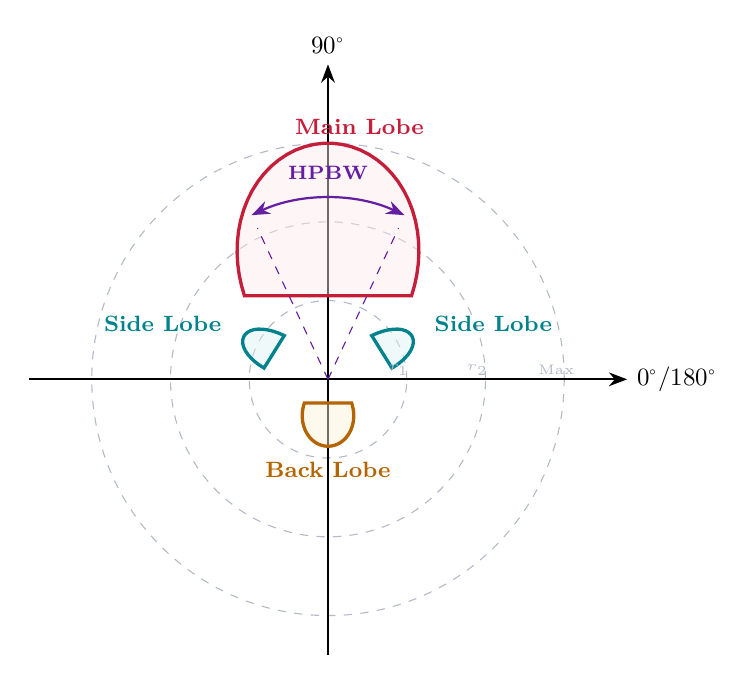
\begin{tikzpicture}[scale=1.0]
  % ── Polar grid ──────────────────────────────────────────────────────────────
  \draw[dashed, color=mgframe, thin] (0,0) circle (1);
  \draw[dashed, color=mgframe, thin] (0,0) circle (2);
  \draw[dashed, color=mgframe, thin] (0,0) circle (3);
  % Axes
  \draw[-Stealth, thick] (-3.8,0) -- (3.8,0) node[right, font=\small] {$0^\circ / 180^\circ$};
  \draw[-Stealth, thick] (0,-3.5) -- (0,4.0) node[above, font=\small] {$90^\circ$};

  % ── Main Lobe (pointing up, $r = 3\cos^2\theta'$, $\theta' = t-90$) ─────────
  \draw[very thick, color=myred, fill=hdrred, fill opacity=0.45, domain=45:135, samples=40, variable=\t]
    plot ({3*cos(\t-90)*cos(\t-90)*cos(\t)}, {3*cos(\t-90)*cos(\t-90)*sin(\t)}) -- cycle;

  % ── Side Lobes ────────────────────────────────────────────────────────────
  % Right side lobe
  \draw[very thick, color=myteal, fill=hdrteal, fill opacity=0.45, domain=10:45, samples=20, variable=\t]
    plot ({1.2*cos(2*(\t-27))*cos(2*(\t-27))*cos(\t)}, {1.2*cos(2*(\t-27))*cos(2*(\t-27))*sin(\t)}) -- cycle;
  % Left side lobe
  \draw[very thick, color=myteal, fill=hdrteal, fill opacity=0.45, domain=135:170, samples=20, variable=\t]
    plot ({1.2*cos(2*(\t-153))*cos(2*(\t-153))*cos(\t)}, {1.2*cos(2*(\t-153))*cos(2*(\t-153))*sin(\t)}) -- cycle;

  % ── Back Lobe ─────────────────────────────────────────────────────────────
  \draw[very thick, color=myamber, fill=hdramber, fill opacity=0.45, domain=225:315, samples=40, variable=\t]
    plot ({0.85*cos(\t-270)*cos(\t-270)*cos(\t)}, {0.85*cos(\t-270)*cos(\t-270)*sin(\t)}) -- cycle;

  % ── HPBW annotation ────────────────────────────────────────────────────────
  \draw[dashed, thin, color=mypurple] (0,0) -- ({2.12*cos(115)},{2.12*sin(115)});
  \draw[dashed, thin, color=mypurple] (0,0) -- ({2.12*cos(65)},{2.12*sin(65)});
  \draw[Stealth-Stealth, thick, color=mypurple]
    ({2.3*cos(115)},{2.3*sin(115)}) arc (115:65:2.3)
    node[midway, above=3pt, font=\scriptsize\bfseries\color{mypurple}] {HPBW};

  % ── Labels ──────────────────────────────────────────────────────────────────
  \node[font=\footnotesize\bfseries\color{myred}] at (0.4, 3.2) {Main Lobe};
  \node[font=\footnotesize\bfseries\color{myteal}] at (2.1, 0.7) {Side Lobe};
  \node[font=\footnotesize\bfseries\color{myteal}] at (-2.1, 0.7) {Side Lobe};
  \node[font=\footnotesize\bfseries\color{myamber}] at (0, -1.15) {Back Lobe};
  % Scale labels
  \node[font=\tiny\color{mgframe}] at (0.9, 0.12) {$r_1$};
  \node[font=\tiny\color{mgframe}] at (1.9, 0.12) {$r_2$};
  \node[font=\tiny\color{mgframe}] at (2.9, 0.12) {Max};
\end{tikzpicture}
\end{tcolorbox}

\subsection{Half-Power Beamwidth (HPBW) and First-Null Beamwidth (FNBW)}
\begin{itemize}[leftmargin=*, itemsep=3pt]
  \item \textbf{Half-Power Beamwidth (HPBW):} The angular width of the main beam between two directions where the radiation intensity is half ($3\,\text{dB}$ below) the maximum value.
  \item \textbf{First-Null Beamwidth (FNBW):} The angular width between the first two nulls (where the radiation intensity drops to zero) on either side of the main beam.
\end{itemize}

\subsection{Antenna Field Regions}
The space surrounding an antenna is divided into three regions depending on the distance $r$ from the antenna. Let $D$ be the maximum dimension of the antenna, and $\lambda$ be the wavelength.

\begin{tcolorbox}[tikzbox, title={Antenna Field Regions}]
\centering
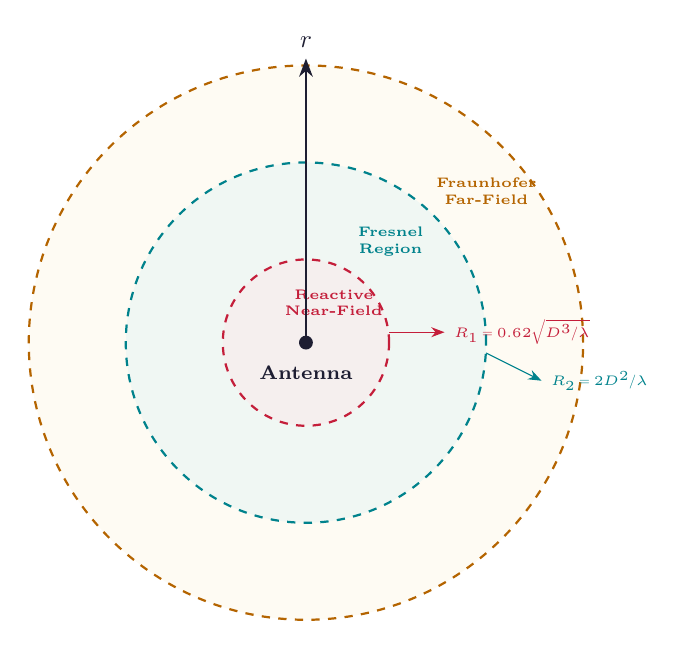
\begin{tikzpicture}[scale=0.88]
  \coordinate (O) at (0,0);

  % Fill regions from outside in (painter's algorithm)
  \fill[hdramber, fill opacity=0.3] (O) circle (4.0);
  \fill[hdrteal, fill opacity=0.4] (O) circle (2.6);
  \fill[hdrred, fill opacity=0.5] (O) circle (1.2);

  % Dashed boundary circles
  \draw[thick, color=myred, dashed] (O) circle (1.2);
  \draw[thick, color=myteal, dashed] (O) circle (2.6);
  \draw[thick, color=myamber, dashed] (O) circle (4.0);

  % Antenna at center
  \fill[mydark] (O) circle (0.1);
  \node[below=5pt, font=\scriptsize\bfseries\color{mydark}] at (O) {Antenna};

  % Region name labels (inside each band)
  \node[align=center, font=\tiny\bfseries\color{myred}] at (55:0.7) {Reactive\\Near-Field};
  \node[align=center, font=\tiny\bfseries\color{myteal}] at (50:1.9) {Fresnel\\Region};
  \node[align=center, font=\tiny\bfseries\color{myamber}] at (40:3.4) {Fraunhofer\\Far-Field};

  % Boundary annotation arrows on horizontal axis
  \draw[thin, -Stealth, color=myred] (1.2, 0.15) -- (2.0, 0.15);
  \node[right, font=\tiny\color{myred}] at (2.0, 0.15) {$R_1 = 0.62\sqrt{D^3/\lambda}$};

  \draw[thin, -Stealth, color=myteal] (2.6, -0.15) -- (3.4, -0.55);
  \node[right, font=\tiny\color{myteal}] at (3.4, -0.55) {$R_2 = 2D^2/\lambda$};

  % Radial axis
  \draw[-Stealth, thick, color=mydark] (0,0) -- (0, 4.1) node[above, font=\small] {$r$};
\end{tikzpicture}
\end{tcolorbox}

\begin{enumerate}[label=\textbf{\arabic*.}, leftmargin=*, itemsep=4pt]
  \item \textbf{Reactive Near-Field Region:} The region immediately surrounding the antenna where the reactive fields (non-radiating, storing energy like a capacitor or inductor) are dominant. The boundary is:
  \[
  r < R_1 = 0.62\sqrt{\frac{D^3}{\lambda}}
  \]
  \item \textbf{Radiating Near-Field (Fresnel) Region:} The region between the reactive near-field and far-field where radiation fields dominate, but the angular field distribution depends on the distance from the antenna (because phase variations across the aperture are significant). The boundary is:
  \[
  0.62\sqrt{\frac{D^3}{\lambda}} \le r < R_2 = \frac{2D^2}{\lambda}
  \]
  \item \textbf{Far-Field (Fraunhofer) Region:} The region where the angular distribution of the electromagnetic fields is independent of the distance. The wave behaves as a local transverse electromagnetic (TEM) plane wave, where the electric and magnetic fields are orthogonal to the direction of propagation. The boundary is:
  \[
  r \ge \frac{2D^2}{\lambda} \quad (\text{provided } D \gg \lambda \text{ and } r \gg \lambda)
  \]
\end{enumerate}

% ===============================================================================
\section{Reciprocity, Directivity, and Gain}
% ===============================================================================

\subsection{Reciprocity Theorem}
The reciprocity theorem states that the electrical characteristics (such as radiation pattern, directivity, input impedance, and effective length) of an antenna remain identical whether it is operated as a transmitter or a receiver.

\textbf{Mathematical Formulation:} Let two antennas $A$ and $B$ exist in a linear, isotropic, and homogenous medium. If a voltage source $V_1$ applied at the terminals of antenna $A$ produces a current $I_2$ at the short-circuited terminals of antenna $B$, and a voltage source $V_2$ applied at the terminals of antenna $B$ produces a current $I_1$ at the short-circuited terminals of antenna $A$, then:
\[
\text{If } V_1 = V_2 \implies I_1 = I_2 \quad (\text{or } Z_{12} = Z_{21})
\]

\subsection{Directivity and Gain}
\begin{itemize}[leftmargin=*, itemsep=3pt]
  \item \textbf{Radiation Intensity ($U$):} The power radiated per unit solid angle (expressed in Watts/steradian).
  \[
  U(\theta, \phi) = r^2 W_{rad}(\theta, \phi)
  \]
  where $W_{rad}$ is the radial component of the Poynting vector.
  \item \textbf{Directivity ($D$):} The ratio of the radiation intensity in a given direction to the average radiation intensity (which is equal to the intensity of an isotropic radiator).
  \[
  D = \frac{U(\theta, \phi)}{U_0} = \frac{4\pi U(\theta, \phi)}{P_{rad}}
  \]
  where $P_{rad} = \int_{0}^{2\pi}\int_{0}^{\pi} U(\theta, \phi) \sin\theta \, d\theta \, d\phi$ is the total radiated power.
  \item \textbf{Gain ($G$):} The ratio of the radiation intensity in a given direction to the radiation intensity that would be obtained if the total power accepted by the antenna ($P_{in}$) was radiated isotropically.
  \[
  G = \frac{4\pi U(\theta, \phi)}{P_{in}}
  \]
  \item \textbf{Relationship between Gain and Directivity:}
  \[
  G = \eta_{cd} D
  \]
  where $\eta_{cd}$ is the antenna radiation efficiency ($0 \le \eta_{cd} \le 1$), representing conduction and dielectric losses.
  \item \textbf{Narrow-Beam Directivity Approximation:} For antennas with a well-defined beam in both principal planes, directivity can be estimated directly from the half-power beamwidths (in degrees):
  \[
  D \approx \frac{41253}{\Theta_{E} \cdot \Theta_{H}}
  \]
  where $\Theta_E$ and $\Theta_H$ are the HPBW in the E-plane and H-plane respectively (in degrees). This formula is accurate to within $\pm 1\,\text{dB}$ for most practical antennas.\end{itemize}

% ===============================================================================
\section{Effective Aperture and Polarization}
% ===============================================================================

\subsection{Effective Aperture (\texorpdfstring{$A_e$}{Ae})}
The \textbf{effective aperture} (or effective area) of a receiving antenna is a measure of its ability to extract power from a passing electromagnetic wave. It is defined as the ratio of the delivered power $P_L$ at the load terminals (matched condition) to the power density $W_{inc}$ of the incident wave.

\begin{tcolorbox}[formulabox, title={\textbf{Effective Aperture and Directivity Relation}}]
The delivered power is $P_L = A_e W_{inc}$. The relationship between the maximum effective aperture $A_{em}$ and the maximum directivity $D_0$ for any antenna is:
\[
A_{em} = \frac{\lambda^2}{4\pi} D_0
\]
\end{tcolorbox}

\subsection{Polarization}
The \textbf{polarization} of an antenna is defined as the polarization of the electromagnetic wave radiated by the antenna in a given direction. It describes the orientation of the electric field vector $\vec{E}$ as a function of time.

There are three main types of polarization:
\begin{itemize}[leftmargin=*, itemsep=3pt]
  \item \textbf{Linear Polarization:} The electric field vector oscillates along a straight line. This occurs when the two orthogonal field components $E_x$ and $E_y$ are in-phase (phase difference $\Delta \psi = 0$ or $180^\circ$).
  \item \textbf{Circular Polarization:} The electric field vector traces out a circle. This requires $E_x = E_y$ and $\Delta \psi = \pm 90^\circ$ ($\pm \pi/2$ rad).
  \item \textbf{Elliptical Polarization:} The electric field vector traces an ellipse. This is the general case when $E_x \neq E_y$ and/or the phase difference is arbitrary (excluding linear/circular conditions).
\end{itemize}

\begin{tcolorbox}[tikzbox, title={Traces of Polarization States}]
\centering
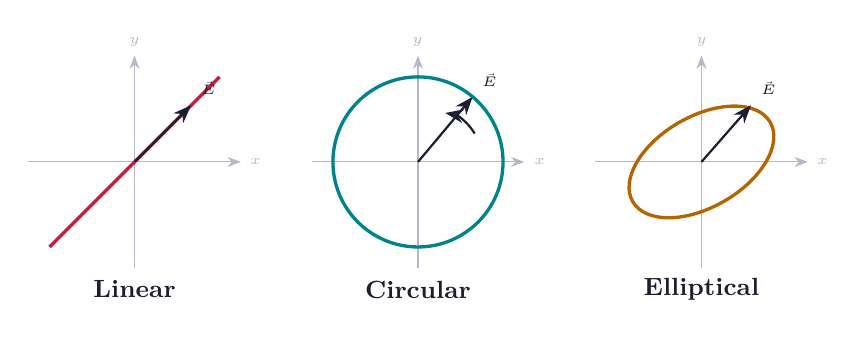
\begin{tikzpicture}[scale=0.9]
  % Linear Polarization
  \begin{scope}[xshift=-4cm]
    \draw[-Stealth, color=mgframe] (-1.5,0) -- (1.5,0) node[right, font=\tiny] {$x$};
    \draw[-Stealth, color=mgframe] (0,-1.5) -- (0,1.5) node[above, font=\tiny] {$y$};
    \draw[very thick, color=myred] (-1.2,-1.2) -- (1.2,1.2);
    \draw[-Stealth, thick, color=mydark] (0,0) -- (0.8,0.8) node[above right, font=\tiny] {$\vec{E}$};
    \node[font=\small\bfseries\color{mydark}] at (0,-1.8) {Linear};
  \end{scope}

  % Circular Polarization
  \begin{scope}[xshift=0cm]
    \draw[-Stealth, color=mgframe] (-1.5,0) -- (1.5,0) node[right, font=\tiny] {$x$};
    \draw[-Stealth, color=mgframe] (0,-1.5) -- (0,1.5) node[above, font=\tiny] {$y$};
    \draw[very thick, color=myteal] (0,0) circle (1.2);
    \draw[-Stealth, thick, color=mydark] (0,0) -- ({1.2*cos(50)}, {1.2*sin(50)}) node[above right, font=\tiny] {$\vec{E}$};
    \draw[-Stealth, thick, color=mydark] (0.8, 0.4) arc (30:80:0.6);
    \node[font=\small\bfseries\color{mydark}] at (0,-1.8) {Circular};
  \end{scope}

  % Elliptical Polarization
  \begin{scope}[xshift=4cm]
    \draw[-Stealth, color=mgframe] (-1.5,0) -- (1.5,0) node[right, font=\tiny] {$x$};
    \draw[-Stealth, color=mgframe] (0,-1.5) -- (0,1.5) node[above, font=\tiny] {$y$};
    \draw[very thick, color=myamber, rotate=30, xscale=1.4, yscale=0.8] (0,0) circle (0.8);
    \draw[-Stealth, thick, color=mydark] (0,0) -- (0.7,0.8) node[above right, font=\tiny] {$\vec{E}$};
    \node[font=\small\bfseries\color{mydark}] at (0,-1.8) {Elliptical};
  \end{scope}
\end{tikzpicture}
\end{tcolorbox}

% ===============================================================================
\section{Input Impedance, Efficiency, and Friis Transmission Equation}
% ===============================================================================

\subsection{Input Impedance}
The \textbf{input impedance} ($Z_{in}$) of an antenna is the impedance presented by the antenna at its terminals. It consists of a real part (input resistance $R_{in}$) and an imaginary part (input reactance $X_{in}$):
\[
Z_{in} = R_{in} + j X_{in}
\]
The input resistance $R_{in}$ is composed of:
\[
R_{in} = R_r + R_L
\]
where $R_r$ is the \textbf{radiation resistance} (representing the power converted into radiated waves) and $R_L$ is the \textbf{loss resistance} (representing conduction and dielectric heating losses).

\subsection{Antenna Efficiency}
The total antenna efficiency ($\eta_0$) accounts for all losses in the system:
\[
\eta_0 = \eta_r \eta_c \eta_d = \eta_r \eta_{cd}
\]
where:
\begin{itemize}[leftmargin=*, itemsep=1pt]
  \item $\eta_r = 1 - |\Gamma|^2$ is the reflection (mismatch) efficiency ($\Gamma$ is the reflection coefficient).
  \item $\eta_c$ is the conduction efficiency.
  \item $\eta_d$ is the dielectric efficiency.
  \item $\eta_{cd} = \eta_c \eta_d = \frac{R_r}{R_r + R_L}$ is the radiation efficiency.
\end{itemize}

\subsection{Friis Transmission Equation}
The Friis transmission equation relates the power received by an antenna ($P_r$) to the power transmitted by another antenna ($P_t$), separated by a distance $r$ in free space.

\begin{tcolorbox}[formulabox, title={\textbf{Friis Transmission Formula}}]
Let $G_t$ be the gain of the transmitting antenna and $G_r$ be the gain of the receiving antenna. The received power is:
\[
P_r = P_t G_t G_r \left( \frac{\lambda}{4\pi r} \right)^{\!2} (PLF)
\]
where $PLF = |\hat{\rho}_t \cdot \hat{\rho}_r|^2$ is the Polarization Loss Factor ($0 \le PLF \le 1$). For matched polarizations, $PLF = 1$.
\end{tcolorbox}

\textbf{Derivation:}
\begin{enumerate}[label=\textbf{\arabic*.}, leftmargin=*, itemsep=3pt]
  \item The power density $W_t$ radiated by an isotropic source at distance $r$ is:
  \[
  W_{isotropic} = \frac{P_t}{4\pi r^2}
  \]
  \item For a directive transmitting antenna with gain $G_t$, the power density in its direction of maximum radiation is:
  \[
  W_t = \frac{P_t G_t}{4\pi r^2}
  \]
  \item The receiving antenna collects this energy using its effective aperture $A_{er}$:
  \[
  P_r = W_t A_{er} = \left( \frac{P_t G_t}{4\pi r^2} \right) A_{er}
  \]
  \item Using the relationship between effective aperture and gain ($A_{er} = G_r \frac{\lambda^2}{4\pi}$):
  \[
  P_r = \left( \frac{P_t G_t}{4\pi r^2} \right) \left( G_r \frac{\lambda^2}{4\pi} \right) = P_t G_t G_r \left( \frac{\lambda}{4\pi r} \right)^{\!2}
  \]
\end{enumerate}

% ===============================================================================
\section{Radiation Integrals and Potential Functions}
% ===============================================================================

To calculate the fields radiated by an antenna, we use auxiliary potential functions rather than solving Maxwell's equations directly. The most common vector potentials are:
\begin{itemize}[leftmargin=*, itemsep=3pt]
  \item $\vec{A}$ (Magnetic Vector Potential): Created by electric current sources $\vec{J}$.
  \item $\vec{F}$ (Electric Vector Potential): Created by magnetic current sources $\vec{M}$ (equivalent currents).
\end{itemize}

\subsection{Relationship between Potentials and Fields}
For a magnetic vector potential $\vec{A}$, the magnetic flux density is:
\[
\vec{B} = \nabla \times \vec{A} \implies \vec{H} = \frac{1}{\mu} \nabla \times \vec{A}
\]
From Maxwell's equation $\nabla \times \vec{E} = -j\omega\mu\vec{H}$, we substitute $\vec{H}$ to get:
\[
\vec{E} = -j\omega\vec{A} - \frac{j}{\omega\mu\epsilon}\nabla(\nabla \cdot \vec{A})
\]

\subsection{Inhomogeneous Helmholtz Wave Equation}
From Maxwell's equations, the potential function $\vec{A}$ satisfies:
\[
\nabla^2 \vec{A} + k^2 \vec{A} = -\mu \vec{J}
\]
where $k = \omega\sqrt{\mu\epsilon} = 2\pi/\lambda$ is the wave number. 

The solution to this inhomogeneous wave equation in free space is:
\[
\vec{A}(x, y, z) = \frac{\mu}{4\pi} \iiint_{V} \vec{J}(x', y', z') \frac{e^{-j k R}}{R} \, dV'
\]
where:
\begin{itemize}[leftmargin=*, itemsep=1pt]
  \item $(x', y', z')$ are the coordinates of the source currents.
  \item $(x, y, z)$ are the coordinates of the observation point.
  \item $R = \sqrt{(x-x')^2 + (y-y')^2 + (z-z')^2}$ is the distance from the source point to the observation point.
\end{itemize}

In the far field, the distance $R$ can be approximated as $R \approx r - r'\cos\psi$ for phase terms, and $R \approx r$ for amplitude terms. This simplifies the vector potential to:
\[
\vec{A} \approx \frac{\mu e^{-jkr}}{4\pi r} \iiint_{V} \vec{J}(x', y', z') e^{jkr'\cos\psi} \, dV'
\]

% ===============================================================================
% MANDATORY QUICK REVISION PAGE
% ===============================================================================
\newpage
\begin{center}
  {\large\bfseries\color{myred} Quick Revision --- Module 1}\\[3pt]
  {\small\color{mydark} Fundamental Concepts of Antennas $|$ PE-EC801A}
\end{center}
\noindent{\color{myred}\rule{\linewidth}{1.2pt}}
\vspace{4pt}

\begin{tcolorbox}[formulabox, title={\textbf{Key Formulas and Metrics at a Glance}}]
\renewcommand{\arraystretch}{1.35}
\begin{tabularx}{\linewidth}{B{5.0cm} X}
Radiation Intensity ($U$) & $U = r^2 W_{rad}$ \quad (Watts/steradian) \\[4pt]
Directivity ($D$) & $D = \frac{4\pi U}{P_{rad}}$ \\[4pt]
Gain ($G$) & $G = \eta_{cd} D = \frac{4\pi U}{P_{in}}$ \\[4pt]
Effective Aperture-Gain Relation & $A_{em} = \frac{\lambda^2}{4\pi} D_0$ \\[4pt]
Narrow-Beam Directivity Approx. & $D \approx \frac{41253}{\Theta_E \cdot \Theta_H}$ \quad ($\Theta$ in degrees) \\[4pt]
Friis Transmission Equation & $P_r = P_t G_t G_r \left( \frac{\lambda}{4\pi r} \right)^{\!2} (PLF)$ \\[4pt]
Helmholtz Equation Solution & $\vec{A} = \frac{\mu}{4\pi} \iiint \vec{J} \frac{e^{-jkR}}{R} dV'$ \\[4pt]
Helmholtz Wave Number ($k$) & $k = \frac{2\pi}{\lambda} = \omega\sqrt{\mu\epsilon}$ \\[4pt]
\end{tabularx}
\end{tcolorbox}

\begin{tcolorbox}[defbox, title={\textbf{One-Line Definitions}}]
\begin{itemize}[leftmargin=*, itemsep=2pt, topsep=0pt]
  \item \textbf{Transducer:} A device that converts energy from one form to another; antennas convert guided electromagnetic waves into free-space waves.
  \item \textbf{Radiation Pattern:} The spatial distribution of physical quantities (like power or field intensity) radiated by an antenna.
  \item \textbf{HPBW:} The angle between the two directions in which the radiation intensity is half of the maximum.
  \item \textbf{Reactive Near-Field:} The region closest to the antenna where reactive non-radiating energy is stored.
  \item \textbf{Far-Field (Fraunhofer) Region:} The region where waves behave as transverse electromagnetic (TEM) plane waves and the pattern does not change with distance.
  \item \textbf{Reciprocity:} The property where transmitting and receiving characteristics of an antenna are identical.
  \item \textbf{Polarization Loss Factor (PLF):} A factor measuring mismatch loss between the polarization of a wave and the receiving antenna.
\end{itemize}
\end{tcolorbox}

\begin{tcolorbox}[exambox, title={\textbf{Frequently Asked / Viva Questions}}]
\begin{enumerate}[topsep=0pt, label=\textbf{Q\arabic*.}, itemsep=5pt]
  \item \Q{What is the physical mechanism of antenna radiation?}
    Radiation is produced by accelerated or decelerated charges, or equivalently, by time-varying currents. Charges oscillating on a conductor generate changing electric and magnetic fields that propagate outward as electromagnetic waves.
  \item \Q{State the three field regions of an antenna and write their boundary equations.}
    \begin{itemize}[leftmargin=*, itemsep=1pt, topsep=2pt]
      \item Reactive near-field: $r < 0.62\sqrt{D^3/\lambda}$
      \item Radiating near-field (Fresnel): $0.62\sqrt{D^3/\lambda} \le r < 2D^2/\lambda$
      \item Far-field (Fraunhofer): $r \ge 2D^2/\lambda$
    \end{itemize}
  \item \Q{Define directivity. How is it different from power gain?}
    Directivity is the ratio of radiation intensity in a given direction to average radiation intensity (purely directional focus). Power gain also accounts for efficiency (conduction and dielectric losses) in addition to directional focus ($G = \eta_{cd} D$).
  \item \Q{State the reciprocity theorem for antennas.}
    The transmitting and receiving properties of an antenna (pattern, impedance, directivity) are identical. A voltage source $V$ at the terminals of antenna $A$ produces current $I$ at antenna $B$, and the same source $V$ at $B$ produces the same current $I$ at $A$.
  \item \Q{What is Polarization Loss Factor (PLF)? What is its value for a vertically polarized antenna receiving a horizontally polarized wave?}
    PLF measures the loss due to polarization mismatch between the incoming wave and the receiving antenna. For orthogonal polarizations (vertical vs. horizontal), $PLF = 0$ (zero power is received).
  \item \Q{Derive the relationship between effective aperture and directivity.}
    Under thermodynamic equilibrium, the ratio of maximum effective aperture to directivity is constant for all antennas: $\frac{A_{em}}{D_0} = \frac{\lambda^2}{4\pi}$. Thus, $A_{em} = \frac{\lambda^2}{4\pi} D_0$.
  \item \Q{Explain the physical meaning of radiation resistance.}
    It is an equivalent resistance that would dissipate the same amount of power as heat as the antenna actually radiates into free space: $R_r = \frac{2 P_{rad}}{I_0^2}$.
  \item \Q{State the Friis transmission equation. What parameters does it relate?}
    $P_r = P_t G_t G_r \left( \frac{\lambda}{4\pi r} \right)^2$. It relates received power ($P_r$) to transmitted power ($P_t$) based on antenna gains ($G_t, G_r$), operating wavelength ($\lambda$), and separation distance ($r$).
  \item \Q{What are auxiliary potential functions? Why are they used?}
    Auxiliary vector potentials ($\vec{A}$ and $\vec{F}$) are mathematical helper functions. They are used because it is much simpler to compute the potentials from the current distributions ($\vec{J}, \vec{M}$) and then take derivatives to get the fields ($\vec{E}, \vec{H}$), rather than solving Maxwell's equations directly.
  \item \Q{Under what conditions does a charge radiate?}
    A charge radiates only if it is accelerated or decelerated. A stationary charge or a charge moving with constant velocity along a straight, infinite transmission line does not radiate.
  \end{enumerate}
\end{tcolorbox}

\begin{tcolorbox}[tikzbox, title={Comparison of Field Regions}]
\centering
\renewcommand{\arraystretch}{1.55}
{\renewcommand{\arraystretch}{1.55}%
\begin{tabularx}{\linewidth}{|B{3.2cm}|Y|Y|Y|}
\hline
\multicolumn{1}{|>{\centering\arraybackslash}m{3.2cm}|}{\textbf{Property}} &
\multicolumn{1}{>{\centering\arraybackslash}Y|}{\textbf{Reactive Near-Field}} &
\multicolumn{1}{>{\centering\arraybackslash}Y|}{\textbf{Radiating Near-Field}} &
\multicolumn{1}{>{\centering\arraybackslash}Y|}{\textbf{Far-Field}} \\
\hline
Dominant Field Type & Reactive fields (energy storage) & Radiating fields (reactive fields decay) & Radiating fields (pure real power) \\
\hline
Pattern Shape & Changes drastically with distance & Varies with distance ($r$) & Independent of distance ($r$) \\
\hline
Phase Fronts & Highly complex & Non-spherical & Spherical (locally planar) \\
\hline
Wave Impedance & Complex (reactive) & Varies & Real ($\approx 377\,\Omega$ in free space) \\
\hline
\end{tabularx}}
\end{tcolorbox}

\end{document}
